\documentclass[runningheads]{llncs}
\usepackage[T1]{fontenc}
\usepackage{amsmath,amssymb}
\usepackage{graphicx}
\usepackage{booktabs}
\usepackage{xcolor}
\usepackage{hyperref}
\hypersetup{colorlinks=true,linkcolor=blue!50!black,citecolor=blue!50!black,urlcolor=blue!50!black}

\newcommand{\Z}{\mathbb{Z}}
\newcommand{\R}{\mathbb{R}}
\newcommand{\conv}{\operatorname{conv}}
\newcommand{\A}{\operatorname{A}}
\newcommand{\dH}{d_H}

\begin{document}
\title{How Round Can a Digital Granulometry Be?}
\titlerunning{How Round Can a Digital Granulometry Be?}
\author{Anonymous Author(s)}
\authorrunning{Anonymous}
\institute{Anonymous Institution}
\maketitle

\begin{abstract}
Granulometries by disks are the standard morphological tool for measuring size distributions, but on $\Z^2$ two of their requirements conflict: the structuring elements should look like Euclidean disks, and they should satisfy Matheron's absorption axiom, i.e.\ each disk must be open with respect to every smaller one. We first show that the digital disks provided by common libraries violate the axiom for most pairs of radii, including most consecutive radii. Families that satisfy it are classically built as Minkowski chains of small structuring elements (neighbourhood sequences, periodic lines, Bresenham decompositions), and they are visibly polygonal. We prove that this is unavoidable: if every element of a Minkowski chain with bounded radius steps lies within Hausdorff distance $\varepsilon$ of a Euclidean disk, then $\varepsilon$ grows at least like $\rho^{1/3}$ with the radius $\rho$, and linearly when the elementary structuring elements come from a fixed finite library. The proof combines the additivity of width functions with an elementary gap property of lattice directions. We complement the bound with constructions. A real-valued relaxation stays numerically bounded up to radius 2000, which points to integrality as the obstruction. Chains of periodic lines with linear-programming weights, and chains computed by mixed-integer programming, roughly halve the error of octagons at practical radii and reduce it tenfold at radius 1000. Experiments on rotated synthetic scenes and on three real images show the effect of these differences on granulometric size distributions, and also where it vanishes.
\keywords{Granulometry \and Digital disk \and Minkowski sum \and Lattice polygon \and Width function \and Pattern spectrum}
\end{abstract}

%===============================================================================
\section{Introduction}
Granulometries, introduced by Matheron~\cite{matheron1975}, formalise sieving: a family of openings $(\gamma_\lambda)_{\lambda\ge0}$ that are decreasing in $\lambda$ and satisfy the absorption law $\gamma_\lambda\gamma_\mu=\gamma_\mu\gamma_\lambda=\gamma_{\max(\lambda,\mu)}$. The size distribution and pattern spectrum derived from them~\cite{maragos1989,serra1982,soille2003} are among the most widely used morphological descriptors. For openings by structuring elements $B_\lambda$, absorption holds if and only if $B_\mu$ is $B_\lambda$-open, i.e.\ a union of translates of $B_\lambda$, for all $\lambda\le\mu$. In $\R^2$ the family of Euclidean disks satisfies this condition, and it is the canonical isotropic granulometry.

On the grid $\Z^2$ the situation is different. The digital disks $\{p\in\Z^2:\|p\|\le r\}$ used by common software are not open with respect to each other in general (Sect.~\ref{sec:violation}): with \texttt{scikit-image}~\cite{vanderwalt2014}, \textbf{73\%} of the pairs of radii up to $40$ violate the condition, as do \textbf{30 out of 39} consecutive pairs. The resulting ``disk granulometries'' are therefore not granulometries. The classical remedy~\cite{adams1993,jones1996,soille2003,vincent1994} is to build structuring elements as \emph{Minkowski chains} $D_k=D_{k-1}\oplus C_k$. Such a family is automatically granulometric, because $D\oplus C$ is $D$-open. The elementary sets $C_k$ come from a small library: the $4$- and $8$-neighbourhoods give octagons (neighbourhood sequences~\cite{rosenfeld1968,farkas2006}), periodic lines~\cite{jones1996}, or Bresenham segments~\cite{adams1993}. These families are polygonal, and their deviation from the disk grows with the radius.

This paper asks how round a granulometric family of digital disks can be, and gives the following answers.
\begin{itemize}
\item \textbf{Lower bound} (Theorem~\ref{thm:lower}). If every element of a Minkowski chain with radius steps at most $\Delta$ is within Hausdorff distance $\varepsilon$ of a Euclidean disk, then $\varepsilon\ge c\,\rho^{1/3}$ at radius $\rho$. With a fixed finite library the error is linear in $\rho$, with an explicit constant computed by linear programming (Corollary~\ref{cor:library}). The proof relies on the additivity of width functions and on a gap in the set of short lattice directions.
\item \textbf{Integrality is the obstruction} (numerically). When the multiplicities of the elementary sets may be real, the best monotone family has error at most $0.43$ for all radii up to $2000$. We prove no such bound for the relaxation (Sect.~\ref{sec:constructions}).
\item \textbf{Constructions.} Chains of periodic lines with linear-programming weights, and chains computed by mixed-integer programming, all with radius steps below $2.2$, have half the error of octagons for $\rho\le48$. Up to $\rho=1000$ the error is $3.7$, against $38$ for octagons and a lower bound of $0.47$ for the same radius steps.
\item \textbf{Experiments.} Gauss disks produce non-monotone size distributions; granulometric chains cannot. Rounder chains are less orientation dependent on polygonal structures, while on three real images the differences fall below the effect of resampling (Sect.~\ref{sec:experiments}).
\end{itemize}
Related work on approximating circles by neighbourhood sequences~\cite{farkas2006} or spheres by zonohedra~\cite{jensen2019} optimises roundness for a fixed library, and Soille and Talbot~\cite{soille2001} noted that radial decompositions by Bresenham lines do not generate granulometries. Our lower bound explains why no choice of library can resolve the conflict.

%===============================================================================
\section{Preliminaries}\label{sec:prelim}
For a finite set $X\subset\Z^2$ and a unit vector $u_\theta=(\cos\theta,\sin\theta)$, the support function is $h_X(\theta)=\max_{p\in X}\langle p,u_\theta\rangle$ and the \emph{width function} is $w_X(\theta)=h_X(\theta)+h_X(\theta+\pi)$, the width of $\conv X$ in direction $u_\theta$. It is translation invariant and $\pi$-periodic, and the diameter of $\conv X$ equals $\max_\theta w_X$. Support functions, hence width functions, are additive under Minkowski addition~\cite{schneider2014}:
\begin{equation}\label{eq:additive}
w_{X\oplus Y}=w_X+w_Y .
\end{equation}
The \emph{anisotropy} of $X$ is $\A(X)=\max_\theta w_X(\theta)-\min_\theta w_X(\theta)$. We say that $X$ is \emph{$\varepsilon$-round with radius $\rho$} if $\dH(\conv X,B(c,\rho))\le\varepsilon$ for some centre $c$. Then $|h_X(\theta)-\langle c,u_\theta\rangle-\rho|\le\varepsilon$, hence
\begin{equation}\label{eq:round}
2\rho-2\varepsilon\le w_X\le2\rho+2\varepsilon\quad\text{and}\quad \A(X)\le4\varepsilon .
\end{equation}

The opening of $Y\subseteq\Z^2$ by a structuring element $D$ is $Y\circ D=\bigcup\{D+t: D+t\subseteq Y\}$. A family of structuring elements $(D_k)$ generates a granulometry if and only if $D_l\circ D_k=D_l$ for all $k\le l$~\cite{matheron1975,serra1982}. Since this relation is transitive, it suffices to check consecutive elements. A \emph{Minkowski chain} is a family with $D_k=D_{k-1}\oplus C_k$ for finite sets $C_k$; every Minkowski chain is granulometric. When all $C_k$ belong to a finite set $\mathcal L$ (up to translation), we call $\mathcal L$ the \emph{library} of the chain.

%===============================================================================
\section{Digital Disks Are Not Granulometric}\label{sec:violation}
We tested the condition ``$D_r$ is $D_s$-open'' for all pairs $1\le s<r\le40$, for the digital disks of \texttt{scikit-image}~\cite{vanderwalt2014} (\texttt{disk(r)}, the Gauss digitisation $\{p:\|p\|\le r\}$) and of OpenCV~\cite{bradski2000} (\texttt{MORPH\_ELLIPSE}). Table~\ref{tab:violation} reports the results. Most pairs violate the condition, including most \emph{consecutive} pairs, so neither family generates a granulometry.

\begin{table}[t]
\centering
\caption{Violations of the absorption condition by standard digital disks, $1\le s<r\le40$.}\label{tab:violation}
\begin{tabular}{lccc}
\toprule
 & violating & violating & images with non-\\
family & pairs $(s,r)$ & pairs $(r-1,r)$ & monotone size distr.\\
\midrule
\texttt{scikit-image} \texttt{disk} & 571/780 (73\%) & 30/39 & 253/400\\
OpenCV \texttt{MORPH\_ELLIPSE} & 628/780 (81\%) & 36/39 & 241/400\\
\bottomrule
\end{tabular}
\end{table}

The consequence is not cosmetic. If $D_r$ is not $D_s$-open, then $X\circ D_r\not\subseteq X\circ D_s$ for some $X$, and the size distribution $r\mapsto|X\circ D_r|$ can \emph{increase}: the pattern spectrum then takes negative values. On random images made of 3 to 11 disks, rectangles or digital disks ($120\times120$ pixels, $r\le15$), this happened for 253 of 400 images. For example, in one image the opened area grows from 2053 to 2089 pixels between $r=8$ and $r=9$. All three of \texttt{scipy.ndimage}, \texttt{scikit-image} and OpenCV agree, up to border conventions. In Sect.~\ref{sec:experiments} the same effect appears on rotated test scenes.

One might hope to extract a granulometric \emph{subsequence} of digital disks. Over all origin-centred digital disks $\{p:\|p\|^2\le n\}$, $n\le900$, we computed the largest radius reachable by a chain of consecutively open disks whose radius gaps are at most $G$. It is $2.0$ for $G=1$, $9.9$ for $G=2$ and $21.8$ for $G=3$, and only with $G\ge5$ is radius $30$ reached. Granulometries made of digital disks are thus necessarily coarse.

%===============================================================================
\section{A Lower Bound for Minkowski Chains}\label{sec:lower}
The key observation is that \eqref{eq:additive} turns roundness of every element of a chain into a constraint on the increments. If $D_{k-1}$ and $D_k$ are both nearly round, then $w_{C_k}=w_{D_k}-w_{D_{k-1}}$ is nearly constant, so $C_k$ has small diameter and all its edges are short lattice vectors. Short lattice vectors leave a gap of directions around each axis, and a polygon whose edges avoid an angular interval cannot be round.

\begin{lemma}[direction gap]\label{lem:gap}
Let $d\ge1$. No nonzero lattice vector $(a,b)$ with $a^2+b^2\le d^2$ has a direction angle in the open interval $(0,\arctan(1/d))$.
\end{lemma}
\begin{proof}
A direction in that interval requires $a>0$ and $b\ge1$, hence $b/a\ge1/a\ge1/d$.\qed
\end{proof}

\begin{theorem}\label{thm:lower}
Let $(D_k)_{k=0}^K$ be a Minkowski chain of finite subsets of $\Z^2$ such that each $D_k$ is $\varepsilon$-round with radius $\rho_k$, and $\rho_k-\rho_{k-1}\le\Delta$ for all $k$. Let $d=2\Delta+4\varepsilon$ and $\alpha=\arctan(1/d)$. Then
\begin{equation}\label{eq:bound}
8\varepsilon\ \ge\ 2\,(\rho_K-\rho_0-2\varepsilon)\,\bigl(1-\cos(\alpha/2)\bigr).
\end{equation}
Consequently, for fixed $\Delta$, $\varepsilon\ge(1-o(1))\,\bigl((\rho_K-\rho_0)/512\bigr)^{1/3}$ as $\rho_K\to\infty$.
\end{theorem}
\begin{proof}
\emph{Step 1 (short increments).} By \eqref{eq:additive} and \eqref{eq:round}, $w_{C_k}=w_{D_k}-w_{D_{k-1}}\le(2\rho_k+2\varepsilon)-(2\rho_{k-1}-2\varepsilon)\le d$. Hence $\operatorname{diam}\conv C_k\le d$, and every edge of the lattice polygon $\conv C_k$ is a lattice vector of norm at most $d$.

\emph{Step 2 (one polygon).} Let $P=\sum_{k=1}^K\conv C_k$ and $Q=\frac12(P-P)$. Then $W:=w_{D_K}-w_{D_0}=w_P=2h_Q$, and $Q$ is a centrally symmetric polygon whose edge directions are among those of the $\conv C_k$. By Lemma~\ref{lem:gap}, no edge direction of $Q$ lies in $(0,\alpha)$. The outer normals of consecutive edges of $Q$ therefore leave an interval $I$ of normal angles of length at least $\alpha$ on which a single vertex $q$ of $Q$ attains the support: $h_Q(\theta)=|q|\cos(\theta-\theta_q)$ for $\theta\in I$.

\emph{Step 3 (anisotropy).} We may assume $\rho_K-\rho_0>2\varepsilon$, since otherwise \eqref{eq:bound} is trivial; then $h_Q>0$ and $|\theta-\theta_q|<\pi/2$ on $I$, and a cosine restricted to an interval of length $\alpha$ varies by at least $1-\cos(\alpha/2)$ times its amplitude. Moreover $|q|\ge\min h_Q=\frac12\min W\ge\rho_K-\rho_0-2\varepsilon$ by \eqref{eq:round}. Hence $\A(W):=\max W-\min W\ge2(\rho_K-\rho_0-2\varepsilon)(1-\cos(\alpha/2))$.

\emph{Step 4.} Finally $\A(W)\le\A(D_K)+\A(D_0)\le8\varepsilon$ by \eqref{eq:round}, which gives \eqref{eq:bound}. For the asymptotic form, $1-\cos(\alpha/2)=\alpha^2/8+O(\alpha^4)$ and $\alpha=1/d+O(d^{-3})$. Since \eqref{eq:bound} forces $\varepsilon\to\infty$ as $\rho_K\to\infty$, we have $d=4\varepsilon(1+o(1))$, and \eqref{eq:bound} becomes $8\varepsilon\ge(\rho_K-\rho_0)/(64\,\varepsilon^2)\,(1+o(1))$.\qed
\end{proof}

The bound uses only the Minkowski structure and integrality: Step~1 is where lattice points enter. It holds for any centres, so the elements need not be concentric, and for any shape of the increments. It is tight in its mechanism: in the real-valued relaxation of Sect.~\ref{sec:constructions}, where Step~1 fails, bounded error appears achievable.

\begin{corollary}[fixed library]\label{cor:library}
Let $\mathcal L$ be a finite library containing at least one set with more than one point, and let
\[
\kappa(\mathcal L)=\min\Bigl\{\tfrac14\A\bigl(\textstyle\sum_{C\in\mathcal L}\lambda_C w_C\bigr)\ :\ \lambda\ge0,\ \min_\theta\textstyle\sum_C\lambda_Cw_C(\theta)=2\Bigr\}.
\]
Then $\kappa:=\kappa(\mathcal L)>0$, and every Minkowski chain with library $\mathcal L$ whose elements are $\varepsilon$-round satisfies $\varepsilon\ge\bigl(\kappa(\rho_K-\rho_0)-\frac14\A(D_0)\bigr)/(1+2\kappa)$, i.e.\ $\varepsilon\ge\frac{\kappa}{1+2\kappa}\rho_K-O(1)$.
\end{corollary}
\begin{proof}
$\sum_C\lambda_Cw_C$ is the width function of the polygon $\sum_C\lambda_C\conv C$, which does not have constant width because bodies of constant width are strictly convex~\cite{schneider2014}. Restricted to the sets of more than one point, the feasible $\lambda$ can be normalised to a compact set on which the anisotropy is continuous and positive, so $\kappa>0$. Write $W=w_{D_K}-w_{D_0}=\sum_Cn_Cw_C$ with multiplicities $n_C$, and $s=\frac12\min W\ge\rho_K-\rho_0-2\varepsilon$ by \eqref{eq:round}. Then $W/s$ is feasible, so $\A(W)\ge4\kappa s$. Combining $\A(W)\le\A(D_K)+\A(D_0)\le4\varepsilon+\A(D_0)$ with $s\ge\rho_K-\rho_0-2\varepsilon$ gives the claim.\qed
\end{proof}

Computing $\kappa(\mathcal L)$ is a linear program on a fine grid of directions. Table~\ref{tab:kappa} lists it for classical libraries: octagons (neighbourhood sequences) lose about $4\%$ of the radius, and every finite library loses a fixed fraction. The corollary is tight for octagons: our best octagon chain has error $38.05$ at $\rho=1000$, matching the leading term $\frac{\kappa}{1+2\kappa}\rho=38.06$ up to the $O(1)$ correction.

\begin{table}[t]
\centering
\caption{Slope $\kappa(\mathcal L)$ of Corollary~\ref{cor:library} for classical libraries: no Minkowski chain built from $\mathcal L$ is better than $\frac{\kappa}{1+2\kappa}\rho-O(1)$ round. $N_4$, $N_8$: $4$- and $8$-neighbourhoods. Segment libraries contain the $D_4$-images of the 8-connected digital straight segments (or of periodic lines~\cite{jones1996}, which have the width function of Euclidean segments) of all primitive vectors of norm $\le m$.}\label{tab:kappa}
\begin{tabular}{lcc@{\qquad}lcc}
\toprule
library & $\kappa$ & $\kappa\cdot100$ & library & $\kappa$ & $\kappa\cdot100$\\
\midrule
$\{N_4\}$ or $\{N_8\}$ & 0.2071 & 20.7 & DSS, $m=\sqrt5$ & 0.0176 & 1.76\\
$\{N_4,N_8\}$ (octagons) & 0.0412 & 4.12 & DSS, $m=5$ & 0.0078 & 0.78\\
periodic lines, $m=\sqrt5$ & 0.0137 & 1.37 & DSS, $m=10$ & 0.0028 & 0.28\\
periodic lines, $m=5$ & 0.0038 & 0.38 & DSS, $m=20$ & 0.0007 & 0.07\\
\bottomrule
\end{tabular}
\end{table}

Two remarks. First, $\kappa(\{N_4\})=(\sqrt2-1)/2$ is the familiar anisotropy of the square. Second, enlarging the library lowers $\kappa$ only quadratically in $m$, as Lemma~\ref{lem:gap} predicts, while Theorem~\ref{thm:lower} shows that an unbounded library does not help either when the radius steps are bounded: the increments must then be short, which re-creates a finite effective library at every scale.

%===============================================================================
\section{Constructions}\label{sec:constructions}
\paragraph{Libraries.} We use three kinds of elementary sets, always together with their images under the dihedral group $D_4$ of the grid. For a primitive vector $v=(a,b)$, $a\ge b\ge0$, these are the 8-connected digital straight segment (DSS)~\cite{klette2004,reveilles1991} $\{(x,\lfloor bx/a+\frac12\rfloor):0\le x\le a\}$, with symmetric rounding of ties, which corresponds to a Bresenham segment~\cite{adams1993}; the two-point periodic line $\{0,v\}$~\cite{jones1996}; and the $2\times2$ square, which every chain contains. A DSS has the extent of a segment plus a lateral thickness of up to one pixel, whereas a periodic line has none. By Corollary~\ref{cor:library} this makes periodic-line libraries rounder: $\kappa=0.0137$ against $0.0176$ for the eight directions of $(1,0),(1,1),(2,1)$ (Table~\ref{tab:kappa}).

\paragraph{Hole-freeness.} A Minkowski sum of digital sets may have holes, i.e.\ lattice points of $\conv(A\oplus B)$ outside $A\oplus B$~\cite{murota2003,murota2023}. Results that exclude holes require compatible normal fans~\cite{haase2008} or $M^\natural$-convexity~\cite{murota2003}, and neither applies here. \emph{None of our results depends on hole-freeness}: the granulometric property holds for any Minkowski chain, and all errors are computed on $\conv D$, using $\conv(A\oplus B)=\conv A+\conv B$. Holes only matter for whether an element can be called a digital disk. We therefore checked every element used in this paper exhaustively, and all are hole-free. This is not automatic: periodic-line chains with $|v|\le6$ do produce holes. Sums of DSS containing the $2\times2$ square were hole-free in all of 700 random trials, and we conjecture that this always holds.

\paragraph{The real relaxation.} Replace the integer multiplicities $n_g$ of the DSS orbits by real numbers $x_g(\rho)\ge0$, non-decreasing in $\rho$. Minimising $\max_\rho\sup_\theta|\sum_gx_g(\rho)h_g(\theta)-\rho|$ over a grid of radii is then a single linear program. Numerically, its optimum stays small: $0.26$ for $|v|\le20$ and $\rho\le400$, $0.34$ for $|v|\le32$ and $\rho\le1000$, and $0.43$ for $|v|\le45$ and $\rho\le2000$. We have not proved that it remains bounded. The optimal real chains use few, long segments with \emph{fractional} multiplicities, which is exactly what Step~1 of Theorem~\ref{thm:lower} rules out for integer chains with bounded steps. This suggests that integrality, not monotonicity, is the obstruction.

\paragraph{Integer chains.} We construct integer chains in two ways, in both cases with radius steps below $2.2$, i.e.\ about one element per integer radius.
(i) \emph{LP-weighted libraries.} For a library $\mathcal L$, let $\lambda^\ast$ be the optimal weights of Corollary~\ref{cor:library}. As $t$ grows, we move towards the multiplicities $\operatorname{round}(t\lambda^\ast)$ one elementary set at a time, choosing at each step the set that keeps the element roundest. By Corollary~\ref{cor:library} the error then grows like $\frac{\kappa}{1+2\kappa}\rho$ plus a rounding term that increases with the library. This scheme also yields the Adams-type (DSS) and periodic-line baselines.
(ii) \emph{MILP.} For radii $r=1,\dots,R$, a mixed-integer program chooses multiplicities $n_{r,g}\in\Z_{\ge0}$ of individual DSS, non-decreasing in $r$, together with a centre, a radius $\rho_r\in[r-\frac12,r+\frac12]$ and an error $t_r$ per element, subject to $|h_{D_r}(\theta)-\langle c_r,u_\theta\rangle-\rho_r|\le t_r$ on 240 directions. It minimises $\max_rt_r$ plus a small multiple of the mean. A look-ahead greedy solution warm-starts HiGHS~\cite{huangfu2018}.

\begin{table}[t]
\centering
\caption{Error $\varepsilon$ (pixels) of families of structuring elements for $\rho\le48$, all with radius steps below $2.2$. The last column gives the largest radius reached with $\max\varepsilon\le1$.}\label{tab:families}
\begin{tabular}{lcccc}
\toprule
family & granulometric & $\max\varepsilon$ & mean $\varepsilon$ & $\rho$ at $\varepsilon\le1$\\
\midrule
Gauss disks (\texttt{disk}) & no & 0.35 & 0.21 & --\\
octagons (neighbourhood seq.) & yes & 1.85 & 0.98 & 25\\
Bresenham/DSS, 8 directions & yes & 3.27 & 1.75 & 12\\
periodic lines, 8 dir., LP weights & yes & 1.09 & 0.60 & 41\\
periodic lines, 13 dir., LP weights & yes & 1.04 & 0.48 & 46\\
DSS, $|v|\le6$, MILP & yes & 1.00 & 0.57 & 44\\
\bottomrule
\end{tabular}
\end{table}

Table~\ref{tab:families} and Fig.~\ref{fig:error}(a) compare the families. The three optimised chains reach about $1.0$ at $\rho=48$, roughly half the error of octagons and a third of that of DSS radial decompositions. Gauss disks remain rounder ($0.35$) but are not granulometric. The step size matters, as Theorem~\ref{thm:lower} predicts through $d=2\Delta+4\varepsilon$: without intermediate steps, the 13-direction periodic chain has radius steps up to $4.1$ and an error of only $0.41$ for $\rho\le48$.

\paragraph{Large radii.} For a fixed library the error grows linearly (Corollary~\ref{cor:library}). Larger libraries have a smaller slope but a larger rounding constant, so the best library depends on the range of radii (Fig.~\ref{fig:error}b). With steps below $3.1$, the best periodic-line chain has error $1.32$ up to $\rho=100$ ($|v|\le\sqrt{10}$), $2.24$ up to $300$ ($|v|\le5$), and $3.73$ up to $1000$ ($|v|\le\sqrt{50}$). For comparison, octagons reach $38.1$, and Theorem~\ref{thm:lower} gives $0.47$ at $\rho=1000$ for the same step size. Closing this gap, which is about a factor of eight at $\rho=1000$, is the main open problem left by this paper. Neither the bound nor the constructions are known to be optimal.

\begin{figure}[t]
\centering
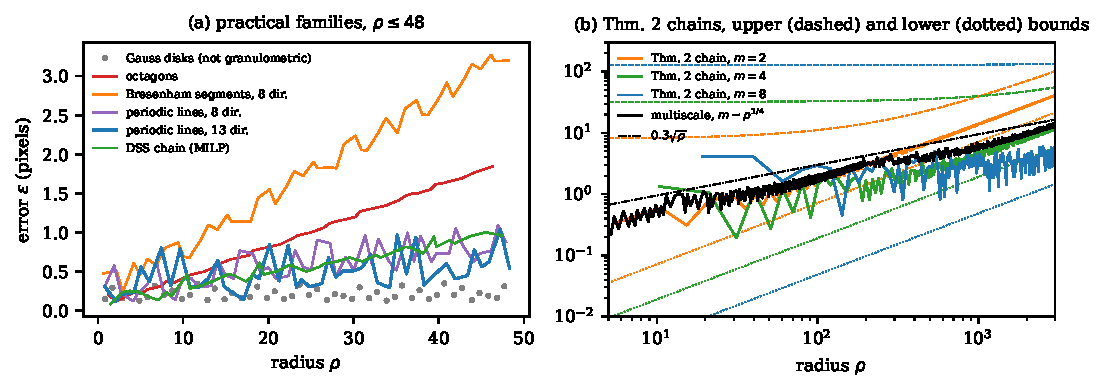
\includegraphics[width=\textwidth]{figures/error.pdf}
\caption{Roundness error of granulometric chains. (a) All families of Table~\ref{tab:families}, $\rho\le48$. (b) Running maximum of the error up to $\rho=1000$ for octagons and LP-weighted periodic-line chains (radius steps below $3.1$); dashed and dotted lines show the bound \eqref{eq:bound}. Gauss disks are not Minkowski chains, so the bound does not apply to them.}\label{fig:error}
\end{figure}

%===============================================================================
\section{Experiments}\label{sec:experiments}
\begin{figure}[t]
\centering
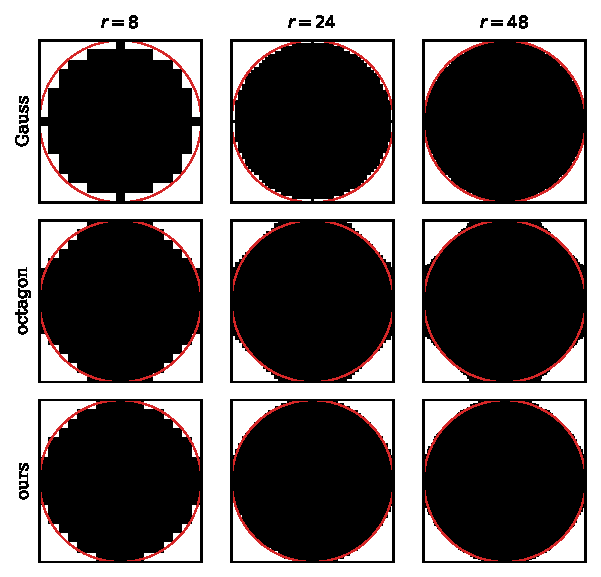
\includegraphics[width=0.62\textwidth]{figures/shapes.pdf}
\caption{Elements at radii 8, 24 and 48, with the best-fitting circle. Gauss digital disks (top) are round but not granulometric; octagons (middle) are granulometric but polygonal; the LP-weighted 13-direction periodic-line chain (bottom) is granulometric and nearly round.}\label{fig:shapes}
\end{figure}

\paragraph{Protocol.} An isotropic granulometry should give the same size distribution for an object and its rotated copies. For each scene $X$ and angle $\theta\in\{0^\circ,5^\circ,\dots,45^\circ\}$, we compute $F_\theta(r)=|X_\theta\circ D_r|/|X_\theta|$ for every family. Openings by chain elements are implemented as cascades of erosions and dilations by their elementary sets, which also makes them fast. We report the rotation sensitivity $S=\operatorname{mean}_r\operatorname{std}_\theta F_\theta(r)$ and the number of increases $F_\theta(r+1)>F_\theta(r)$, which are impossible for a granulometry. The scenes are a synthetic scene of nine squares of sides 17 to 81 pixels, rasterised exactly after rotation ($r\le40$), and three real images from \texttt{scikit-image}~\cite{vanderwalt2014}: fluorescence microscopy of nuclei (\texttt{human\_mitosis}, $r\le15$), \texttt{coins} ($r\le30$) and a material texture (\texttt{gravel}, $r\le20$). Real images are smoothed, rotated with bilinear interpolation and thresholded at the Otsu level of the unrotated image.

\begin{table}[t]
\centering
\caption{Rotation sensitivity $S$ ($\times10^{3}$) of size distributions; in parentheses, the number of increases of $F_\theta$ when nonzero.}\label{tab:rotation}
\begin{tabular}{lcccccc}
\toprule
scene & Gauss & octagons & DSS 8 dir. & periodic 8 & periodic 13 & DSS MILP\\
\midrule
squares (synthetic) & 4.0 (17) & 30.2 & 13.3 & 11.8 & 9.5 & 17.6\\
nuclei (microscopy) & 1.7 & 1.9 & 1.9 & 2.0 & 1.6 & 1.4\\
coins & 5.0 & 5.0 & 6.4 & 4.2 & 5.0 & 6.2\\
gravel & 1.4 & 1.3 & 1.6 & 1.1 & 1.6 & 1.2\\
\bottomrule
\end{tabular}
\end{table}

\begin{figure}[t]
\centering
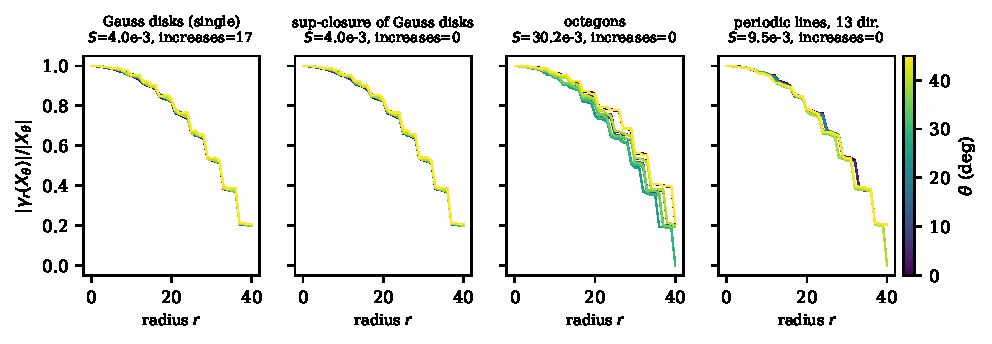
\includegraphics[width=\textwidth]{figures/rotation.pdf}
\caption{Size distributions of the rotated synthetic scene, one curve per angle. Gauss disks are nearly isotropic but non-monotone; octagons are monotone but orientation dependent; the periodic-line chain is monotone and three times less orientation dependent than octagons.}\label{fig:rotation}
\end{figure}

\paragraph{Results.} Table~\ref{tab:rotation} and Fig.~\ref{fig:rotation} summarise the results. On the synthetic scene, Gauss disks are the least orientation dependent but produce 17 increases of the size distribution, i.e.\ negative pattern-spectrum values. Octagons are monotone but strongly orientation dependent ($S=30.2\cdot10^{-3}$): the curves for $\theta=0^\circ$ and $\theta\approx22^\circ$ separate as soon as the squares no longer contain the octagons in both orientations. The 13-direction periodic-line chain divides this by three. On the three real images, the families differ by at most $0.6\cdot10^{-3}$ (nuclei, gravel) and $2.2\cdot10^{-3}$ (coins), with no consistent ranking, i.e.\ within the effect of interpolation and thresholding, and no increases occur. Their objects are rounded and randomly oriented, so the anisotropy of the structuring element is averaged out. The practical benefit of round granulometric chains is therefore largest for polygonal or aligned structures. The violation of the axiom by Gauss disks is a correctness issue that can surface on any image (Table~\ref{tab:violation}).

%===============================================================================
\section{Conclusion}
Digital disks as provided by standard libraries do not generate granulometries. The classical granulometric replacements, Minkowski chains, cannot be uniformly round: with bounded radius steps their error grows at least like $\rho^{1/3}$, and linearly for any fixed library, with a slope that we compute exactly. The real relaxation appears to admit bounded error, which suggests that integrality is the obstruction. LP-weighted periodic-line chains and MILP chains halve the error of octagons at practical radii and reduce it tenfold at $\rho=1000$, but a gap of about a factor of eight to the lower bound remains. Three questions are open: the optimal growth rate for Minkowski chains; whether granulometries that are not Minkowski chains, where $D_l$ is merely a union of translates of $D_k$, can be uniformly round; and whether sums of digital segments containing a $2\times2$ square are always hole-free. Extensions to $\Z^3$, where Lemma~\ref{lem:gap} has a direct analogue, are natural.

\bibliographystyle{splncs04}
\bibliography{refs}
\end{document}
